%\documentclass[prd,twocolumn,aps,psfig,showpacs,nofootinbib,nobibnotes,superscriptaddress,preprintnumbers,times]{revtex4}
\documentclass[prd,twocolumn,aps,psfig,nofootinbib,nobibnotes,superscriptaddress,preprintnumbers,times]{revtex4-2}
\setlength{\topmargin}{-14mm}
\usepackage{graphicx,bm,color,hyperref,amsmath,amssymb, mathtools,subcaption, float,dblfloatfix}
\graphicspath{{./fig/}}

\def\red{\textcolor{red}}
\def\blue{\textcolorFujita:2018}

%|||||||||||||||||||||||||||||||||||||||||||||||||||||||||||||||||||
%             Customized Commands
%|||||||||||||||||||||||||||||||||||||||||||||||||||||||||||||||||||
%  mathematical abbreviations
%
%
%
\newcommand{\BoldVec}[1]{\mathchoice%
  {\mbox{\boldmath $\displaystyle     #1$}}%
  {\mbox{\boldmath $\textstyle        #1$}}%
  {\mbox{\boldmath $\scriptstyle      #1$}}%
  {\mbox{\boldmath $\scriptscriptstyle#1$}}%
}
%\newcommand{\BoldVec}[1]{\bm{#1}}}
%
% math debs
\newcommand{\EQ}{\begin{equation}}
\newcommand{\EN}{\end{equation}}
\newcommand{\EQA}{\begin{eqnarray}}
\newcommand{\ENA}{\end{eqnarray}}
\newcommand{\eq}[1]{(\ref{#1})}
\newcommand{\EEq}[1]{Equation~(\ref{#1})}
\newcommand{\Eq}[1]{Eq.~(\ref{#1})}
\newcommand{\Eqs}[2]{Eqs~(\ref{#1}) and~(\ref{#2})}
\newcommand{\EEqs}[2]{Equations~(\ref{#1}) and~(\ref{#2})}
\newcommand{\eqs}[2]{(\ref{#1}) and~(\ref{#2})}
\newcommand{\Eqss}[2]{Eqs~(\ref{#1})--(\ref{#2})}
%\newcommand{\Sec}[1]{\S\,\ref{#1}}
%\newcommand{\Secs}[2]{\S\S\,\ref{#1} and~\ref{#2}}
\newcommand{\Sec}[1]{Sec.~\ref{#1}}
\newcommand{\Secs}[2]{Secs.~\ref{#1} and~\ref{#2}}
\newcommand{\App}[1]{Appendix~\ref{#1}}
\newcommand{\Fig}[1]{Fig.~\ref{#1}}
\newcommand{\FFig}[1]{Figure~\ref{#1}}
\newcommand{\Tab}[1]{Table~\ref{#1}}
\newcommand{\Figs}[2]{Figs.~\ref{#1} and \ref{#2}}
\newcommand{\Tabs}[2]{Tables~\ref{#1} and \ref{#2}}
%\newcommand{\bra}[1]{\langle #1\rangle}
\newcommand{\bbra}[1]{\left\langle #1\right\rangle}
\newcommand{\mean}[1]{\overline #1}
\newcommand{\meanB}{\overline{B}}
\newcommand{\meanC}{\overline{C}}
\newcommand{\meanU}{\overline{U}}
\newcommand{\meanW}{\overline{W}}
\newcommand{\meanPhi}{\overline{\Phi}}
\newcommand{\meanF}{\overline{\cal F}}
\newcommand{\meanR}{\overline{\cal R}}
\newcommand{\meanAA}{\overline{\bm{A}}}
\newcommand{\meanBB}{\overline{\bm{B}}}
\newcommand{\meanEE}{\overline{\bm{E}}}
\newcommand{\meanUU}{\overline{\bm{U}}}
\newcommand{\meanWW}{\overline{\bm{W}}}
\newcommand{\meanJJ}{\overline{\mbox{\boldmath $J$}}}
\newcommand{\meanuu}{\overline{\mbox{\boldmath $u$}}}
\newcommand{\meanGG}{\overline{\mbox{\boldmath $G$}}}
\newcommand{\meanAB}{\overline{\mbox{\boldmath $A\cdot B$}}}
\newcommand{\meanAoBo}{\overline{\mbox{\boldmath $A_0\cdot B_0$}}}
\newcommand{\meanApoBpo}{\overline{\mbox{\boldmath $A'_0\cdot B'_0$}}}
\newcommand{\meanApBp}{\overline{\mbox{\boldmath $A'\cdot B'$}}}
\newcommand{\meanuxB}{\overline{\mbox{\boldmath $\delta u\times \delta B$}}}
\newcommand{\meanemfs}{\overline{\cal E} {}}
\newcommand{\meanemf}{\overline{\mbox{\boldmath ${\cal E}$}} {}} %redundant
\newcommand{\meanAAAA}{\overline{\mbox{\boldmath ${\mathsf A}$}} {}}
\newcommand{\meanSSSS}{\overline{\mbox{\boldmath ${\mathsf S}$}} {}}
\newcommand{\meanAAA}{\overline{\mathsf{A}}}
\newcommand{\meanSSS}{\overline{\mathsf{S}}}
\newcommand{\meanCC}{\overline{\mbox{\boldmath ${\cal C}$}} {}}
\newcommand{\meanFF}{\overline{\mbox{\boldmath ${\cal F}$}} {}}
\newcommand{\meanRR}{\overline{\mbox{\boldmath ${\cal R}$}} {}}
\newcommand{\calFF}{\overline{\mbox{\boldmath ${\cal F}$}} {}}
\newcommand{\meanEMF}{\overline{\mbox{\boldmath ${\cal E}$}} {}}
\newcommand{\tildeFFFF}{\tilde{\mbox{\boldmath ${\cal F}$}}{}}{}
\newcommand{\hatFFFF}{\hat{\mbox{\boldmath ${\cal F}$}}{}}{}
\newcommand{\meanFFFF}{\overline{\mbox{\boldmath ${\cal F}$}}{}}{}
\newcommand{\meanFFF}{\overline{\cal F}}
\newcommand{\hatOO}{\hat{\bm{\Omega}}}
\newcommand{\hatAA}{\hat{\bm{A}}}
\newcommand{\hatBB}{\hat{\bm{B}}}
\newcommand{\tildeh}{\tilde{h}}
\newcommand{\tildeT}{\tilde{T}}
\newcommand{\tildehhh}{\tilde{\sf h}}
\newcommand{\tildeTTT}{\tilde{\sf T}}
%
% tilde
%
\newcommand{\eee}{{\sf e}}
\newcommand{\hhh}{{\sf h}}
\newcommand{\TTT}{{\sf T}}
\newcommand{\tildexx}{\tilde{\bm{x}}}
\newcommand{\tildeBB}{\tilde{\bm{B}}}
\newcommand{\tildeJJ}{\tilde{\bm{J}}}
\newcommand{\tildeA}{\tilde{A}}
\newcommand{\tildeB}{\tilde{B}}
\newcommand{\tildeJ}{\tilde{J}}
\newcommand{\tildeemf}{\tilde{\cal E}}
\newcommand{\teps}{\tilde{\epsilon} {}}
\newcommand{\tkapz}{\tilde{\kappa_0}}
\newcommand{\Oh}{\hat{\Omega}}
\newcommand{\zh}{\hat{z}}
\newcommand{\PC}{{\sc Pencil Code}~}
\newcommand{\PCS}{{\sc Pencil Code}}
%
%  unit vectors
%
\newcommand{\nullvector}{{\bf0}}
\newcommand{\nnn}{\hat{\mbox{\boldmath $n$}} {}}
\newcommand{\vvv}{\hat{\mbox{\boldmath $v$}} {}}
\newcommand{\rr}{\hat{\mbox{\boldmath $r$}} {}}
\newcommand{\xxx}{\hat{\mbox{\boldmath $x$}} {}}
\newcommand{\yyy}{\hat{\mbox{\boldmath $y$}} {}}
\newcommand{\zz}{\hat{\mbox{\boldmath $z$}} {}}
\newcommand{\pp}{\hat{\mbox{\boldmath $\phi$}} {}}
\newcommand{\ttt}{\hat{\mbox{\boldmath $\theta$}} {}}
\newcommand{\OOO}{\hat{\mbox{\boldmath $\Omega$}} {}}
\newcommand{\ooo}{\hat{\mbox{\boldmath $\omega$}} {}}
\newcommand{\BBBB}{\hat{\mbox{\boldmath $B$}} {}}
\newcommand{\kunit}{\hat{\mbox{$k$}} {}}
\newcommand{\nunit}{\hat{\mbox{$n$}} {}}
%
%  hatted quantities
%
\newcommand{\hatU}{\hat{U}}
\newcommand{\hatUU}{\hat{\bm{U}}}
%
%  vectors
%
\newcommand{\gggg}{\BoldVec{g} {}}
\newcommand{\ddd}{\BoldVec{d} {}}
\newcommand{\rrr}{\BoldVec{r} {}}
\newcommand{\xx}{\BoldVec{x}{}}
\newcommand{\yy}{\BoldVec{y} {}}
\newcommand{\zzz}{\BoldVec{z} {}}
\newcommand{\uu}{\BoldVec{u} {}}
\newcommand{\vv}{\BoldVec{v} {}}
\newcommand{\ww}{\BoldVec{w} {}}
\newcommand{\mm}{\BoldVec{m} {}}
\newcommand{\PP}{\BoldVec{P} {}}
\newcommand{\QQ}{\BoldVec{Q} {}}
\newcommand{\RR}{\BoldVec{R} {}}
\newcommand{\UU}{\BoldVec{U} {}}
\newcommand{\bb}{\BoldVec{b} {}}
\newcommand{\qq}{\BoldVec{q} {}}
\newcommand{\BB}{\BoldVec{B} {}}
\newcommand{\HH}{\BoldVec{H} {}}
\newcommand{\II}{\BoldVec{I} {}}
\newcommand{\AAA}{\BoldVec{A} {}}
\newcommand{\aaa}{\BoldVec{a} {}}
\newcommand{\aaaa}{\BoldVec{a} {}} %(convert aaa -> aaaa, compatibility problem)
%\newcommand{\eee}{\BoldVec{e} {}}
\newcommand{\jj}{\BoldVec{j} {}}
\newcommand{\JJ}{\BoldVec{J} {}}
\newcommand{\nn}{\BoldVec{n} {}}
\newcommand{\ee}{\BoldVec{e} {}}
\newcommand{\ff}{\BoldVec{f} {}}
\newcommand{\hh}{\BoldVec{h} {}}
\newcommand{\EE}{\BoldVec{E} {}}
\newcommand{\FF}{\BoldVec{F} {}}
\newcommand{\TT}{\BoldVec{T} {}}
\newcommand{\CC}{\BoldVec{C} {}}
\newcommand{\KK}{\BoldVec{K} {}}
\newcommand{\MM}{\BoldVec{M} {}}
\newcommand{\GG}{\BoldVec{G} {}}
\newcommand{\kk}{\BoldVec{k} {}}
\newcommand{\SSS}{\BoldVec{S} {}}
\newcommand{\grav}{\BoldVec{g} {}}
\newcommand{\nab}{\BoldVec{\nabla} {}}
\newcommand{\OO}{\BoldVec{\Omega} {}}
\newcommand{\oo}{\BoldVec{\omega} {}}
\newcommand{\LL}{\BoldVec{\Lambda} {}}
\newcommand{\llambda}{\BoldVec{\lambda} {}}
\newcommand{\pomega}{\BoldVec{\varpi} {}}
%
%  correlation tensors
%
\newcommand{\RRRR}{\bm{\mathsf{R}}}
\newcommand{\SSSS}{\bm{\mathsf{S}}}
\newcommand{\LLLL}{\mbox{\boldmath ${\sf L}$} {}}
\newcommand{\MMMM}{\bm{\mathsf{M}}}
\newcommand{\BBB}{\mbox{\boldmath ${\cal B}$} {}}
\newcommand{\emf}{\mbox{\boldmath ${\cal E}$} {}}
\newcommand{\FFF}{\mbox{\boldmath ${\cal F}$} {}}
\newcommand{\GGG}{\mbox{\boldmath ${\cal G}$} {}}
\newcommand{\HHH}{\mbox{\boldmath ${\cal H}$} {}}
\newcommand{\QQQ}{\mbox{\boldmath ${\cal Q}$} {}}
%
%  operators  (roman)
%
\newcommand{\ii}{{\rm i}}
\newcommand{\grad}{{\rm grad} \, {}}
\newcommand{\curl}{{\rm curl} \, {}}
\newcommand{\dive}{{\rm div}  \, {}}
\newcommand{\Dive}{{\rm Div}  \, {}}
\newcommand{\diag}{{\rm diag}  \, {}}
\newcommand{\DD}{{\rm D} {}}
\newcommand{\dd}{{\rm d} {}}
\newcommand{\const}{{\rm const}  {}}
\newcommand{\crit}{{\rm crit}  {}}
\def\degr{\hbox{$^\circ$}}
\def\la{\mathrel{\mathchoice {\vcenter{\offinterlineskip\halign{\hfil
$\displaystyle##$\hfil\cr<\cr\sim\cr}}}
{\vcenter{\offinterlineskip\halign{\hfil$\textstyle##$\hfil\cr<\cr\sim\cr}}}
{\vcenter{\offinterlineskip\halign{\hfil$\scriptstyle##$\hfil\cr<\cr\sim\cr}}}
{\vcenter{\offinterlineskip\halign{\hfil$\scriptscriptstyle##$\hfil\cr<\cr\sim\cr}}}}}
\def\ga{\mathrel{\mathchoice {\vcenter{\offinterlineskip\halign{\hfil
$\displaystyle##$\hfil\cr>\cr\sim\cr}}}
{\vcenter{\offinterlineskip\halign{\hfil$\textstyle##$\hfil\cr>\cr\sim\cr}}}
{\vcenter{\offinterlineskip\halign{\hfil$\scriptstyle##$\hfil\cr>\cr\sim\cr}}}
{\vcenter{\offinterlineskip\halign{\hfil$\scriptscriptstyle##$\hfil\cr>\cr\sim\cr}}}}}
%
%  numbers
%
\def\Ta{\mbox{\rm Ta}}
\def\Ra{\mbox{\rm Ra}}
\def\Ma{\mbox{\rm Ma}}
\def\Sh{\mbox{\rm Sh}}
\def\Roo{\mbox{\rm Ro}^{-1}}
\def\Pra{\mbox{\rm Pr}}
\def\Pran{\mbox{\rm Pr}}
\def\Pm{\mbox{\rm Pr}_{\rm M}}
\def\Rm{\mbox{\rm Re}_{\rm M}}
\def\Rey{\mbox{\rm Re}}
\def\Imag{\mbox{\rm Im}}
\def\Pe{\mbox{\rm Pe}}
\def\epsK{\epsilon_{\rm K}}
\def\epsM{\epsilon_{\rm M}}
\def\EEi{{\cal E}_i}
\def\EEK{{\cal E}_{\rm K}}
\def\EEM{{\cal E}_{\rm M}}
\def\EEKM{{\cal E}_{\rm K/M}}
\def\EEGW{{\cal E}_{\rm GW}}
\def\OmK{{\Omega}_{\rm K}}
\def\OmM{{\Omega}_{\rm M}}
\def\OmGW{{\Omega}_{\rm GW}}
\def\hrms{{h}_{\rm rms}}
\def\EEtot{{\cal E}_{\rm tot}}
\def\EErad{{\cal E}_{\rm rad}}
\def\EElam{{\cal E}_\lambda}
\def\EEcrit{{\cal E}_{\rm crit}}
\def\HHGW{{\cal H}_{\rm GW}}
\def\HHK{{\cal H}_{\rm K}}
\def\HHM{{\cal H}_{\rm M}}
\def\EGW{E_{\rm GW}}
\def\HGW{H_{\rm GW}}
\def\EK{E_{\rm K}}
\def\EM{E_{\rm M}}
\def\HM{H_{\rm M}}
\def\hc{h_{\rm c}}
\def\cs{c_{\rm s}}
\def\xiM{\xi_{\rm M}}
\def\xiK{\xi_{\rm K}}
\def\kf{k_{\rm f}}
%\def\kf{k_\ast}
\def\vA{v_{\rm A}}
\def\urms{u_{\rm rms}}
\def\Urms{U_{\rm rms}}
\def\Brms{B_{\rm rms}}
\def\kappaOO{\kappa_{\Omega\Omega}}
\def\kappaO{\kappa_{\Omega}}
\def\kappat{\kappa_{\rm t}}
\def\kappatz{\kappa_{\rm t0}}
\def\nut{\nu_{\rm t}}
\def\etatz{\eta_{\rm t0}}
\def\etat{\eta_{\rm t}}
\def\etaT{\eta_{\rm T}}
\def\Beq{B_{\rm eq}}
\def\tmax{t_{\max}}
%
\newcommand{\ea}{{\em et al. }}
\newcommand{\eaa}{{\em et al. }}
\def\half{{\textstyle{1\over2}}}
\def\threehalf{{\textstyle{3\over2}}}
\def\onethird{{\textstyle{1\over3}}}
\def\twothird{{\textstyle{2\over3}}}
\def\fourthird{{\textstyle{4\over3}}}
\def\quarter{{\textstyle{1\over4}}}
%
\newcommand{\W}{\,{\rm W}}
\newcommand{\V}{\,{\rm V}}
\newcommand{\kV}{\,{\rm kV}}
\newcommand{\MeV}{\,{\rm MeV}}
\newcommand{\GeV}{\,{\rm GeV}}
\newcommand{\T}{\,{\rm T}}
\newcommand{\uG}{\,\mu{\rm G}}
\newcommand{\G}{\,{\rm G}}
\newcommand{\Hz}{\,{\rm Hz}}
\newcommand{\mHz}{\,{\rm mHz}}
\newcommand{\nHz}{\,{\rm nHz}}
\newcommand{\uHz}{\,\mu{\rm Hz}}
\newcommand{\kHz}{\,{\rm kHz}}
\newcommand{\kG}{\,{\rm kG}}
\newcommand{\K}{\,{\rm K}}
\newcommand{\g}{\,{\rm g}}
\newcommand{\s}{\,{\rm s}}
\newcommand{\ms}{\,{\rm ms}}
\newcommand{\cm}{\,{\rm cm}}
\newcommand{\m}{\,{\rm m}}
\newcommand{\km}{\,{\rm km}}
\newcommand{\kms}{\,{\rm km/s}}
\newcommand{\kg}{\,{\rm kg}}
\newcommand{\Mm}{\,{\rm Mm}}
\newcommand{\pc}{\,{\rm pc}}
\newcommand{\kpc}{\,{\rm kpc}}
\newcommand{\Mpc}{\,{\rm Mpc}}
\newcommand{\yr}{\,{\rm yr}}
\newcommand{\Myr}{\,{\rm Myr}}
\newcommand{\Gyr}{\,{\rm Gyr}}
\newcommand{\erg}{\,{\rm erg}}
\newcommand{\mol}{\,{\rm mol}}
\newcommand{\dyn}{\,{\rm dyn}}
\newcommand{\J}{\,{\rm J}}
\newcommand{\RM}{\,{\rm RM}}
\newcommand{\AU}{\,{\rm AU}}
\newcommand{\A}{\,{\rm A}}
%
\def\hX{h_\times}
\def\hT{h_+}
\def\thT{\tilde{h}_+}
\def\thX{\tilde{h}_\times}
\def\dhT{\dot{h}_+}
\def\dhX{\dot{h}_\times}
\def\dhhT{\dot{\hat{h}}_+}
\def\dhhX{\dot{\hat{h}}_\times}
\def\dhhTX{\dot{\hat{h}}_{+/\times}}
\def\dthT{\dot{\tilde{h}}_+}
\def\dthX{\dot{\tilde{h}}_\times}
\def\dthTX{\dot{\tilde{h}}_{+/\times}}
%
%  journals
%
\newcommand{\arXiv}[3]{, ``#3,'' arXiv:#2 (#1).}
\newcommand{\yjcap}[3]{, J.\ Cosmol.\ Astropart.\ Phys. {\bf #2} (#1) #3.}
\newcommand{\yjas}[3]{, J. Atmosph. Sci. {\bf #2}, #3 (#1).}
\newcommand{\yan}[3]{, Astron. Nachr. {\bf #2}, #3 (#1).}
\newcommand{\yact}[3]{, Acta Astron. {\bf #2}, #3 (#1).}
\newcommand{\yana}[3]{, Astron. Astrophys. {\bf #2}, #3 (#1).}
\newcommand{\yanas}[3]{, Astron. Astrophys. Suppl. {\bf #2}, #3 (#1).}
\newcommand{\yanal}[3]{, Astron. Astrophys. Lett. {\bf #2}, #3 (#1).}
\newcommand{\yass}[3]{, Astrophys. Spa. Sci. {\bf #2}, #3 (#1).}
\newcommand{\ysci}[3]{, Science {\bf #2}, #3 (#1).}
\newcommand{\ysph}[3]{, Solar Phys. {\bf #2}, #3 (#1).}
\newcommand{\yjetp}[3]{, Sov. Phys. JETP {\bf #2}, #3 (#1).}
\newcommand{\yspd}[3]{, Sov. Phys. Dokl. {\bf #2}, #3 (#1).}
\newcommand{\ysov}[3]{, Sov. Astron. {\bf #2}, #3 (#1).}
\newcommand{\ysovl}[3]{, Sov. Astron. Lett. {\bf #2}, #3 (#1).}
\newcommand{\ymn}[3]{, Mon.\ Not.\ R.\ Astron.\ Soc.\ {\bf #2}, #3 (#1).}
\newcommand{\ymhd}[3]{, Magnetohydrohydrodyn. {\bf #2}, #3 (#1).}
\newcommand{\yqjras}[3]{, Quart. J. Roy. Astron. Soc. {\bf #2}, #3 (#1).}
\newcommand{\ynat}[3]{, Nature {\bf #2}, #3 (#1).}
\newcommand{\yjfm}[4]{, ``#4,'' J. Fluid Mech. {\bf #2}, #3 (#1).}
\newcommand{\pjfm}[1]{, J. Fluid Mech., in press (#1).}
\newcommand{\sjfm}[1]{, J. Fluid Mech., submitted (#1).}
\newcommand{\ypr}[3]{, Phys.\ Rev.\ {\bf #2}, #3 (#1).}
\newcommand{\yprd}[4]{, ``#4,'' Phys.\ Rev.\ D {\bf #2}, #3 (#1).}
\newcommand{\ypre}[3]{, Phys.\ Rev.\ E {\bf #2}, #3 (#1).}
\newcommand{\yprf}[4]{, ``#4,'' Phys.\ Rev.\ Fluids {\bf #2}, #3 (#1).}
\newcommand{\yprl}[4]{, ``#4,'' Phys.\ Rev.\ Lett.\ {\bf #2}, #3 (#1).}
\newcommand{\yphl}[3]{, Phys.\ Lett.\ {\bf #2}, #3 (#1).}
\newcommand{\pprl}[1]{, Phys. Rev. Lett., in press (#1).}
\newcommand{\yepl}[3]{, Europhys. Lett. {\bf #2}, #3 (#1).}
\newcommand{\pcsf}[2]{, Chaos, Solitons \& Fractals, in press (#1).}
\newcommand{\ycsf}[3]{, Chaos, Solitons \& Fractals{\bf #2}, #3 (#1).}
\newcommand{\yprs}[3]{, Proc. Roy. Soc. Lond. {\bf #2}, #3 (#1).}
\newcommand{\yptrs}[3]{, Phil. Trans. Roy. Soc. {\bf #2}, #3 (#1).}
\newcommand{\yptrsa}[4]{, ``#4,'' Phil. Trans. Roy. Soc. Lond. A, {\bf #2}, #3 (#1).}
\newcommand{\yjcp}[3]{, J. Comp. Phys. {\bf #2}, #3 (#1).}
\newcommand{\yjgr}[3]{, J. Geophys. Res. {\bf #2}, #3 (#1).}
\newcommand{\ygrl}[3]{, Geophys. Res. Lett. {\bf #2}, #3 (#1).}
\newcommand{\yobs}[3]{, Observatory {\bf #2}, #3 (#1).}
\newcommand{\yaj}[3]{, Astronom. J. {\bf #2}, #3 (#1).}
\newcommand{\sapj}[3]{, ``#3,'' Astrophys. J., submitted, arXiv:#2  (#1).}
\newcommand{\papj}[3]{, ``#3,'' Astrophys. J., in press, arXiv:#2  (#1).}
\newcommand{\yapj}[4]{, ``#4,'' Astrophys. J. {\bf #2}, #3 (#1).}
\newcommand{\yapjs}[3]{, Astrophys. J. Suppl. {\bf #2}, #3 (#1).}
\newcommand{\yapjl}[3]{, Astrophys. J. {\bf #2}, #3 (#1).}
\newcommand{\ycqg}[3]{, Class. Quant. Grav. {\bf #2}, #3 (#1).}
\newcommand{\ypp}[3]{, Phys. Plasmas {\bf #2}, #3 (#1).}
\newcommand{\yppcf}[3]{, Plasmas Phys. Contr. Fusion {\bf #2}, #3 (#1).}
\newcommand{\ppp}[1]{, Phys. Plasmas, in press (#1).}
\newcommand{\ypasj}[3]{, Publ. Astron. Soc. Japan {\bf #2}, #3 (#1).}
\newcommand{\ypac}[3]{, Publ. Astron. Soc. Pacific {\bf #2}, #3 (#1).}
\newcommand{\yaraa}[3]{, Ann. Rev. Astron. Astrophys. {\bf #2}, #3 (#1).}
\newcommand{\yanar}[3]{, Astron. Astrophys. Rev. {\bf #2}, #3 (#1).}
\newcommand{\yanp}[3]{, Ann. Phys. {\bf #2}, #3 (#1).}
\newcommand{\yanf}[3]{, Ann. Rev. Fluid Dyn. {\bf #2}, #3 (#1).}
\newcommand{\ypf}[4]{, ``#4,'' Phys. Fluids {\bf #2}, #3 (#1).}
\newcommand{\yphy}[3]{, Physica {\bf #2}, #3 (#1).}
\newcommand{\ygafd}[4]{, ``#4,'' Geophys. Astrophys. Fluid Dyn. {\bf #2}, #3 (#1).}
\newcommand{\yrpp}[3]{, Rep. Prog. Phys. {\bf #2}, #3 (#1).}
\newcommand{\yptp}[3]{, Progr. Theor. Phys. {\bf #2}, #3 (#1).}
\newcommand{\yjour}[5]{, ``#5,'' #2 {\bf #3}, #4 (#1).}
\newcommand{\pjour}[3]{, #2, in press (#1).}
\newcommand{\sjour}[3]{, #2, submitted (#1).}
\newcommand{\yprep}[2]{, #2, preprint (#1).}
\newcommand{\pproc}[3]{, (ed. #3), #2 (#1) (to appear).}
\newcommand{\yproc}[4]{, (ed. #4), pp. #2. #3 (#1).}
\newcommand{\ybook}[3]{, {\em #2}. #3 (#1).}
\newcommand{\neff}{N_{\rm eff}}
\newcommand{\dneff}{\Delta N_{\rm eff}}
\newcommand{\neffv}{N_{\rm eff}^{(\nu)}}

\usepackage{braket}

\begin{document}

\title{Constraining Models of Massive Gravity Using the NANOGrav 15-Year Data Set}

\date{\today}
\preprint{N/A}
%TK: alphabetic order for now
\author{Chris~Choi}
\email{minyeonc@andrew.cmu.edu}
\affiliation{Department of Physics, Carnegie Mellon University, Pittsburgh, PA 15213, USA}

\author{Murman~Gurgenidze}
\email{mgurgeni@andrew.cmu.edu}
\affiliation{Department of Physics, Carnegie Mellon University, Pittsburgh, PA 15213, USA}

\author{Tina~Kahniashvili}
\email{tinatin@andrew.cmu.edu}
\affiliation{McWilliams Center for Cosmology and Department of Physics, Carnegie Mellon University, Pittsburgh, PA 15213, USA}
\affiliation{School of Natural Sciences and Medicine, Ilia State University, 0194 Tbilisi, Georgia}
\affiliation{Abastumani Astrophysical Observatory, Tbilisi, GE-0179, Georgia}

\author{Jacob~Magallanes}
\email{jmagalla@andrew.cmu.edu}
\affiliation{Department of Physics, Carnegie Mellon University, Pittsburgh, PA 15213, USA}

\begin{abstract}
Convincing evidence of a stochastic gravitational wave background has been found by the NANOGrav collaboration in 15-Year data set \cite{Agazie:2023}. From this signal, we can evaluate the possibility of its source being from the early universe through the tensor perturbations induced by a massive spin-2 graviton field. We consider time independent and time dependent models of massive gravity \cite{Fujita:2018,Gumrukcuoglu:2012}, and compare their energy spectra with the signals from the NANOGrav data. We then place bounds on the mass of the gravitons and bounds on the rate of inflation. We show that the stochastic background allows for the possibility of time dependent massive gravity model to explain the data, within 2 - 4 $\sigma$ deviation, but a suppression mechanism for high frequency modes has to be introduced to obey the BBN bounds. For the time independent model, we find that the lack of a peaked signature in the spectrum allows us to bring the mass bound to $m_g \lesssim 8.3 \GeV/c^2$, in agreement with previous work \cite{deRham:2017,Wang:2023, Wu:2023}.
\end{abstract}

\maketitle

\section{Introduction}
Ever since the discovery of a stochastic gravitational wave background (SGWB) based on the data from 15 years of observation of pulsars by the North American Nanohertz Observatory for Gravitational Waves (NANOGrav) collaboration \cite{Agazie:2023}, there have been attempts to search for new physics in the data \cite{Afzal:2023}. General relativity (GR) is an extremely accurate theory for most of the things we observe, but there are things it cannot presently explain. Many alternate theories of gravity have been proposed to try to address this, including massive gravity (MG), first introduced by Fierz and Pauli in 1939 \cite{Fierz:1939ix}. Massive gravity helps address the source of dark energy; why there is a late time acceleration of the universe at all. It would be quite remarkable if a simple\footnote{The modification by a non-zero graviton mass is actually much more difficult than at first glance, due to the Boulware-Deser ghost and other problems showing up for nonlinear formulations of MG which prevent the theory from reducing to GR in the massless limit, and only recently have they been addressed \cite{Hassan:2012a, Hassan:2012b}} modification to a spin-2 field is the explanation behind such a significant phenomenon. 

In this paper, we will use the 15-year NANOGrav data set (hereafter NG15), to constrain two models of massive gravity: one where the mass is time-independent and one that where the mass is time independent, specifically one where the mass takes the form of a step-function of time. The former will be taken from Ref.\ \cite{Gumrukcuoglu:2012} (hereafter the Constant Mass (CM) model) and the latter will be taken from Ref.\ \cite{Fujita:2018} (hereafter the Step Function Mass (SFM) model). We will calculate the energy density of primordial gravitational waves created during or before inflation, at the present time, and compare them to the signals we observe in NG15. There are multiple lines of evidence that point to the existence of a SGWB, and while many believe the background is mainly due to binary systems of supermassive black holes dispersed throughout the universe, more exotic cosmological sources cannot be excluded  from consideration\cite{Agazie:2023}, including the possibility that the background is due to massive gravity. 
    
The more commonly studied time-independent model has the graviton with a constant, non-zero mass since at least a Planck time after the Big Bang, after the graviton coupled to the Higgs field. There have been bounds placed on the mass of the graviton in such a model \cite{deRham:2017,Wang:2023, Wu:2023}, using the initial Laser Interferometer Gravitational-Wave Observatory (LIGO) detections and NG15. We will take into account these mass bounds and place further bounds for this model, if they are to try to explain the NG15 signals.

The goal of this paper is to show whether massive gravity, through the amplification of tensor modes of primordial gravitational waves that entered the cosmological horizon before the matter dominated era, is a plausible mechanism for generating the SGWB that we observe. 

\section{Setup} 
We start with defining the FLRW metric $g_{\mu\nu}$, which we write as
\begin{equation}\label{eqn:-1}
    g_{\mu\nu}dx^{\mu} dx^{\nu} = -N^2(t)dt^2 +a^2(t)\left(\frac{dr}{1-Kr^2} + r^2 d\Omega^2\right)\ ,
\end{equation}
where $K$ is the spatial curvature, $d\Omega^2 = d\theta^2 + \sin^2\theta d\phi^2$, $N(t)$ is the lapse, and $a(t)$ is the scale factor. We then consider the general Lorentz-invariant action for a massive spin-2 field \cite{Blasi:2017}
\begin{equation}\label{eqn:0}
    S = S_{inv} + S_{m}
\end{equation}

where $S_{inv}$ is the Einstein-Hilbert action defined by 
\begin{equation} \label{eqn:1}
     \begin{multlined}
     S_{inv} = \int \text{d}^4x\Bigg(\frac{1}{2}h\partial^2h - h_{\mu \nu}\partial^\mu \partial^\nu h \\ - \frac{1}{2}h^{\mu\nu} \partial^2 h_{\mu\nu} + h^{\mu\nu}\partial_\nu \partial^\rho h_{\mu \rho} \Bigg) 
    \end{multlined}
\end{equation} 
where $h_{\mu\nu} = h_{\mu\nu}(\tau,{\bf x})$ is the metric perturbation and $\tau$ is the conformal time defined by $\tau \equiv \int \frac{N(t)}{a(t)}dt$, and $S_m$ is the massive action defined by 
\begin{equation} \label{eqn:2}
     \begin{multlined}
     S_m = \int d^4x\frac{1}{2}(m_1^2 h^{\mu\nu}h_{\mu\nu}+ m_2^2 h^2).
    \end{multlined}
\end{equation}
where $m_1$ and $m_2$ are the mass terms defined in Eq.\ 2.3 of \cite{Blasi:2017}. 
We decompose the spatial component of the tensor perturbation $h_{ij}$ into its helicity states like Eq.\ 19.214 of \cite{Maggiore:v2} 
\begin{equation}\label{eqn:3}
    h_{ij}(\tau, {\bf k}) = \sum_{\lambda \in \{+, \times\}}e^\lambda_{ij}(\hat{\bf k})\gamma_k^\lambda(\tau, {\bf k})
\end{equation}
where ${\bf k}$ is the comoving momentum, $e^\lambda_{ij}$ is the polarization tensor given in Eqs. 1.54-56 of \cite{Maggiore:v1}. 
After we minimize the action from Eq.\ \ref{eqn:0} and take into account the helicity decomposition, we obtain the equation of motion (EoM) for $\gamma_{k}^\lambda$ (with the helicity modes suppressed since they have the same EoM)
\begin{equation}\label{eqn:4}
    \overline{\gamma}_k'' + \left(c_g^2(\tau) k^2 + a^2 M_{GW}^2 - \frac{a''}{a} + 2Kc_g^2(\tau)\right)\overline{\gamma}_k = 0
\end{equation}
where $a$ is the scale factor, $\overline{\gamma}_k = a\gamma_k$ is defined for convenience, the primes ($\,'$) denote derivatives with respect to $\tau$, and $c_g(\tau)$ is the effective sound speed associated with GWs and may be dependent on time. For this paper, we will set $K = 0$ and $c_g = 1$. 

\subsection{CM}
In the CM model, the graviton mass is much lower than the Hubble scale during inflation. This means that we don't need to consider the evolution of the GWs during inflation. The scale factor will be taken from solving
\begin{equation}
    \tau = \int \frac{da}{a^2H} = \int \frac{da}{a^2H_0\sqrt{\frac{\Omega_r}{a^4} + \frac{\Omega_m}{a^3}+ \frac{\Omega_k}{a^2}+\Omega_\Lambda}}
    \label{eqn:5}
\end{equation} where $H_0 = H(\tau_0) $ is the Hubble parameter at the present time and is $\approx 2.18\times 10^{-18}$ Hz, and $\Omega_r,$ $ \Omega_m,$ $ \Omega_k, $ $\Omega_\Lambda$ are the present-day density parameters of radiation, matter, curvature, and the cosmological constant respectively. We will take their values to be $8.5\times 10^{-5}$, 0.3, 0, and 0.7 respectively.

We will take the mass function to be $M_{GW} = M_{GW,0}$. 

\subsection{SFM}
We consider graviton masses on the order of the Hubble scale, and so the evolution of the GWs during inflation will be important.
The scale factor, as described in Eq.\ (4) of \cite{Fujita:2018}, is
\begin{equation}
    a(\tau) = 
    \begin{cases}
            -1(H_{\inf}\tau) & \tau < \tau_r \\
            a_r \tau/\tau_r & \tau > \tau_r \\
   \end{cases}
   \label{eqn:6} 
\end{equation}
where $H_{\inf}$ is the Hubble parameter during inflation when the scale corresponding to the Cosmic Microwave Background (CMB) exits the Hubble horizon and $a_r$ is the scale factor at the reheating time $\tau_r = 1/(a_r H_{\inf})$. We will assume $\tau_r$ to be fixed in this discussion, while $H_{\inf}$ and $a_r$ may vary. The bounds on $H_{\inf}$ are discussed in \cite{Jiang:2017}, and they will be respected in this paper. The scale factor in this model has a peculiar behavior where it is not defined in the region $(-\tau_r, \tau_r)$ and only takes values outside of that interval. This is to allow for the scale factor and its first derivative to be continuous. 
\begin{figure}[h]
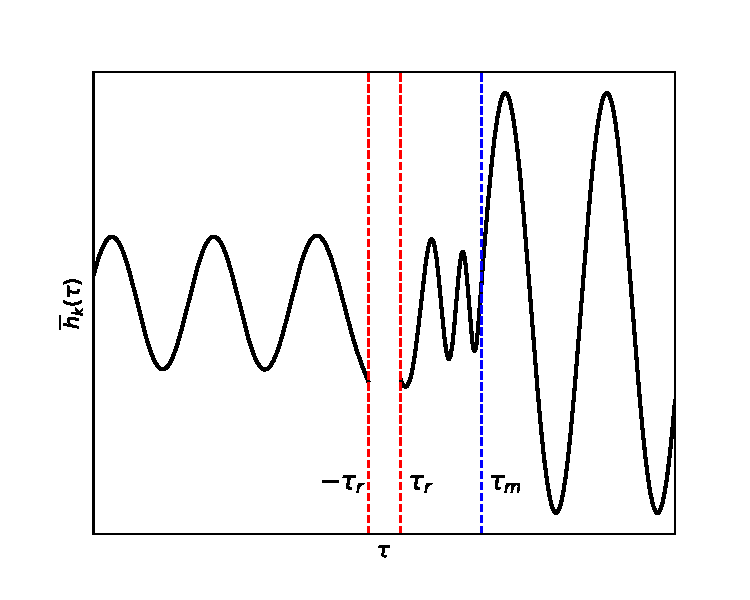
\includegraphics[scale=0.65]{fig/fig0.pdf}
\caption{A schematic of the real part of the mode function $\overline{\gamma}_k(\tau)$. There is a gap in the domain of the conformal time from $-\tau_r$ to $\tau_r$, but the mode function and its first derivative remains continuous in that domain. This is a numerical solution to the differential equation in Eq.\ \ref{eqn:4}, and the exact values for the parameters are detailed in the code \cite{GH}}
\label{fig:mode}
\end{figure}

Fig.\ \ref{fig:mode} illustrates how a generic mode function would look like, showing  the discontinuity in the conformal time. The behavior in the 3 regions of $\tau$ are discussed in detail in \cite{Fujita:2018}.
We will use the mass function from Eq.\ 5 of \cite{Fujita:2018}
\begin{equation}
    M_{GW}(\tau) = 
    \begin{cases}
            m & \tau < \tau_m \\
            0 & \tau > \tau_m \\
   \end{cases}
   \label{eqn:7}
\end{equation} 
where $\tau_m$ is some conformal time during the radiation dominated era when the mass instantaneously drops to 0. For more discussion about why the time is chosen to be in the radiation dominated era, refer to footnote 2 of \cite{Fujita:2018}. 

\section{Energy Density}
When we study models of gravitation, we often want to know how sub-horizon GWs from the primordial era are influenced. The energy density spectrum of these GWs at the present time as a function of frequency is perhaps the most practical way to observe the effects of beyond-GR theories. We want to look at the energy fraction of the GWs per logarithmic interval of k at the current time. We have the following definition for the energy density 
\begin{equation}\label{eqn:8}
    \Omega_{GW} = \frac{1}{\rho_c}\frac{d \rho_{GW}} {d \log{k}}
\end{equation}
where $\rho_c = \frac{3H^2}{8\pi G}$ is the critical density, and we note that the derivative isn't literally with respect to $\log k$ but is notationally representing the spectral density of $\rho_{GW}$ (see footnote 65 of \cite{Maggiore:v1}). Our energy density today is defined in terms of the primordial tensor power spectrum $\mathcal{P}_0(f)$ as detailed in Eq.\ 19.288 of \cite{Maggiore:v2}
\begin{equation}\label{eqn:9}
    \Omega_{GW,0}(f) = \frac{\pi^2}{3a_0^2H_0^2}f^2 \mathcal{P}_0(f)
\end{equation}
where $a_0 = a(\tau_0) = 1$. We will find the power spectrum in MG for both models by finding the form of the enhancement factor that will amplify the GR power spectrum using different approaches.  
\subsection{CM}
The EoM from Eq.\ \ref{eqn:5} yields the dispersion relation
\begin{equation}\label{eqn:10}
    \omega^2 = \frac{k^2}{a^2} + M_{GW}^2\ .
\end{equation}
 For a given mode, if $\omega^2 \gg H^2$, where $H(a)$ is the Hubble parameter, then it is sub-horizon and if $\omega^2 \ll H^2$, then it is super-horizon. A sub-horizon mode will decay with time, and a super-horizon mode will remain fixed since the mode is "frozen" while it is outside the horizon. This is characterized by the equality  
 \begin{equation}\label{eqn:11}
     \omega^2(\tau_k) = H^2(\tau_k)
 \end{equation} where $\tau_k$ is the conformal time at which the mode reenters the horizon for a particular $k$. The scale factor for which is occurs at is notated as $a_k$. In the case of a massless graviton, i.e. the GR case, we have that $\omega = \frac{k}{a}$ and the scale factor for which $\omega(a) = H(a)$ is denoted as $a_{k}^{GR}$ (and similarly with the other parameters $\tau_k^{GR}$).

Ref.\ \cite{Gumrukcuoglu:2012} defines the power spectrum in Eq.\ 39
\begin{equation}\label{eqn:12}
    \mathcal{P}(\omega_0)= \frac{\omega_0^2}{\omega_0^2 - M_{GW,0}^2}\frac{2k^3}{\pi^2}|\gamma_k(\tau_0)|^2
\end{equation}
where $\omega_0 = \omega(\tau_0)$ and $k$ is parametrically defined by $\omega_0$ as
\begin{equation}\label{eqn:13}
    k = a_0 \sqrt{\omega_0^2 -  M_{GW,0}^2} \ .
\end{equation}
where $k' = a_0 \omega_0$. We can write the power spectrum in terms of the enhancement factor $S$ as
\begin{equation}\label{eqn:14}
    \frac{\mathcal{P}(\omega_0)}{\mathcal{P}_{GR}(\omega_0)} = \frac{\mathcal{P}_{prim}(k)}{\mathcal{P}_{prim}(k')}S^2(\omega_0)\ ,
\end{equation}
where $S$ is defined as 
\begin{equation}\label{eqn:15}
    S(\omega_0) = \frac{k' a_k}{k a_{k'}^{GR}} \sqrt{\frac{\omega_k a_k}{\omega_0 a_0}}\ ,
\end{equation}
and where $\omega_k = \sqrt{(k/a_k)^2 + M_{GW}^2}$. $\mathcal{P}_{prim}(k)$ is the primordial power spectrum defined as 
\begin{equation}\label{eqn:16}
    \mathcal{P}_{prim}(k) \equiv \frac{2k^3}{\pi^2}A^2(k)
\end{equation}and is normalized to the constant $2.43\times 10^{-10}$. $A(k)$ is the amplitude of the mode at the time of its generation defined as $A(k) = H_*/(M_{pl} k^{3/2})$ where $H_*$ is the Hubble expansion rate of the horizon exit during inflation and $M_{pl}$ is the reduced Planck mass defined by $M_{pl} = (8\pi G)^{-1/2}$. The GR spectrum is obtained through the WKB approximation in Eq.\ 44 of \cite{Gumrukcuoglu:2012}
\begin{equation}\label{eqn:17}
    \mathcal{P}_{GR}(\omega_0) =  \left( \frac{a_{k'}^{GR}}{a_0}\right)^2 \mathcal{P}_{prim}(k')\ .
\end{equation}
Thus, we see that the power spectrum takes on the form 
\begin{equation}\label{eqn:18}
    \begin{multlined}
    \mathcal{P}(\omega_0)  = \frac{\omega_0 a_k^3 \omega_k}{k^2 a_0} P_{prim}(k)\ .
    \end{multlined}
\end{equation}
It remains to actually compute $a_k$. Ref.\ \cite{Gumrukcuoglu:2012} uses approximations for different regimes of $k$, but we can try to compute it numerically from Eq.\ \ref{eqn:9}. In its expanded form, we are essentially trying to solve 
\begin{equation}\label{eqn:19}
    \frac{k^2}{a_k^2} + M_{GW}^2 = H_0^2\left(\frac{\Omega_r}{a_k^4} + \frac{\Omega_m}{a_k^3}+ \frac{\Omega_k}{a_k^2}+\Omega_\Lambda\right) \ .
\end{equation}This is a quartic in $a_k$ and therefore has an analytic solution, but in our experimentation, we discovered that using the analytical form, provided by Mathematica \cite{Mathematica:2023}, produces wildly inaccurate solutions due to the complexity of the expression and how the errors accumulate. Instead, we are able to use the Python package \texttt{SymPy} \cite{SymPy:2017} to calculate numerical approximations of the roots.

\begin{figure}[h]
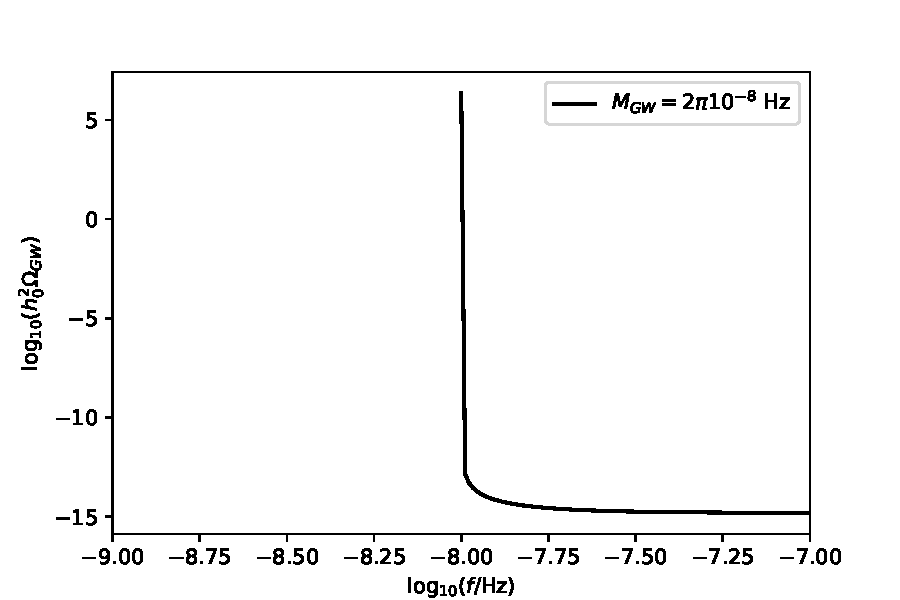
\includegraphics[scale=.565]{fig/fig6.pdf}
\caption{The energy density in the CM model due to a graviton mass of $2\pi 10^{-8}$ Hz. The peak is located at $10^{-8}$ Hz.}
\label{fig:CM_omega}
\end{figure}

When we compute the energy density due to MG in this model, we observe no signal below the cutoff frequency, located at $f = 2\pi\times M_{GW}$. We also see a vertical peak that asymptotically approaches a flat spectrum in the log-log scale. The peak is estimated by Eq.\ 64 of \cite{Gumrukcuoglu:2012}.

\subsection{SFM}

The power spectrum is found to be approximately
\begin{equation}\label{eqn:20}
    \mathcal{P}(\tau, k) \sim \frac{\tau_m}{\tau_r}(k\tau_r)^{3-2\nu}\mathcal{P}_{GR}(\tau,k)\ , 
\end{equation}
where $\mathcal{P}_{GR}$ is the power spectrum of the massless tensor modes from inflation, and $\nu$ is defined by 
\begin{equation}\label{eqn:21}
    \nu = \sqrt{\frac{9}{4} - \frac{m^2}{H_{\inf}^2}}\ .
\end{equation}
This expression for the power spectrum is found by solving the equation of motion for the mode function and finding the expression for $\overline{\gamma}_k$ deep in the massless phase (see Sec.\ III(iii) of \cite{Fujita:2018} for more details). We want to make sure that we respect the Higuchi bound, which is determined by preventing the expression inside the square root from becoming negative: $M_{GW}/H_{\inf} \leq 3/2$. As for the GR power spectrum, we can approximate it by using the transfer function detailed in \cite{Kuroyanagi:2015}. To briefly recount, the power spectrum in the GR case is
\begin{equation}\label{eqn:22}
    \mathcal{P}_{GR} = \mathcal{P}^{prim}_{T} T^2_T(k)
\end{equation}
where $\mathcal{P}^{prim}_{T}$ is the primordial tensor power spectrum and $T_{T}$ is the transfer function describing the standard reheating scenario in which the universe had a short matter-dominated era after inflation before reheating ended. $\mathcal{P}^{prim}_{T}$ is defined 
in Eq.\ 7 of \cite{Kuroyanagi:2015} as follows

\begin{equation}\label{eqn:23}
    \mathcal{P}_{T}^{prim}(k) = A_T(k_{ref})\left(\frac{k}{k_{ref}}\right)^{n_T}
\end{equation}
\begin{figure}[H]
\begin{subfigure}{.5\textwidth}
  \centering
  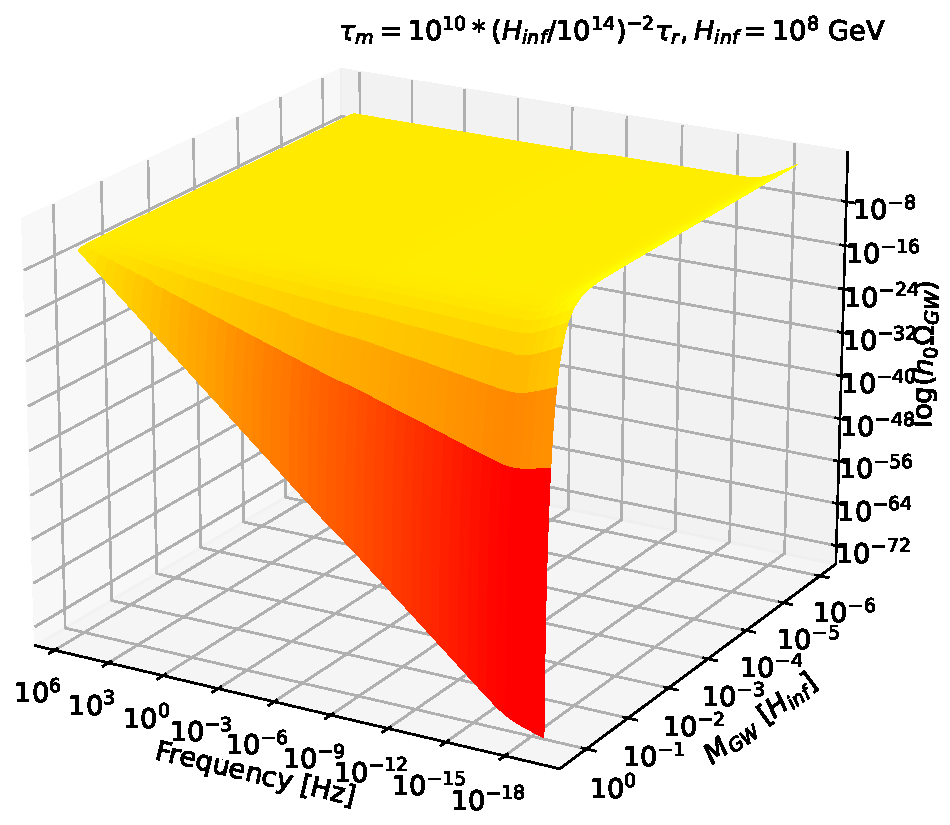
\includegraphics[width=.82\linewidth]{fig/fig4a.pdf}  
  \label{fig:contour-a}
\end{subfigure}
\begin{subfigure}{.5\textwidth}
  \centering
  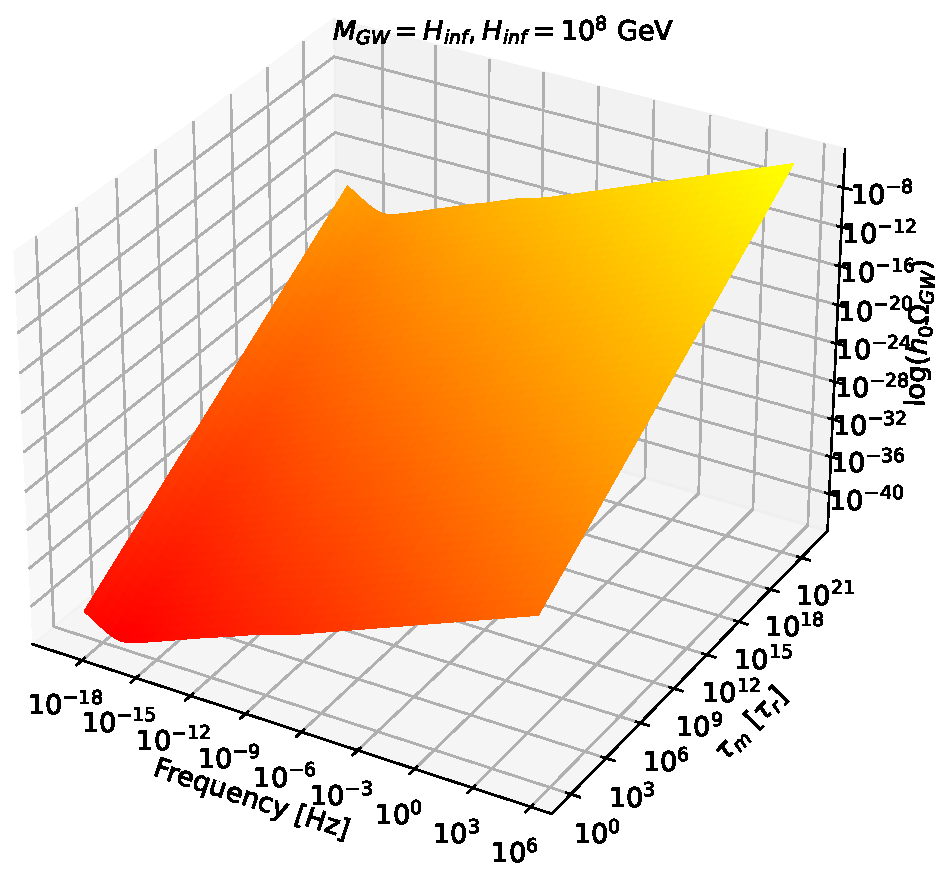
\includegraphics[width=.82\linewidth]{fig/fig4b.pdf}  
  \label{fig:contour-b}
\end{subfigure}
\begin{subfigure}{.5\textwidth}
  \centering
  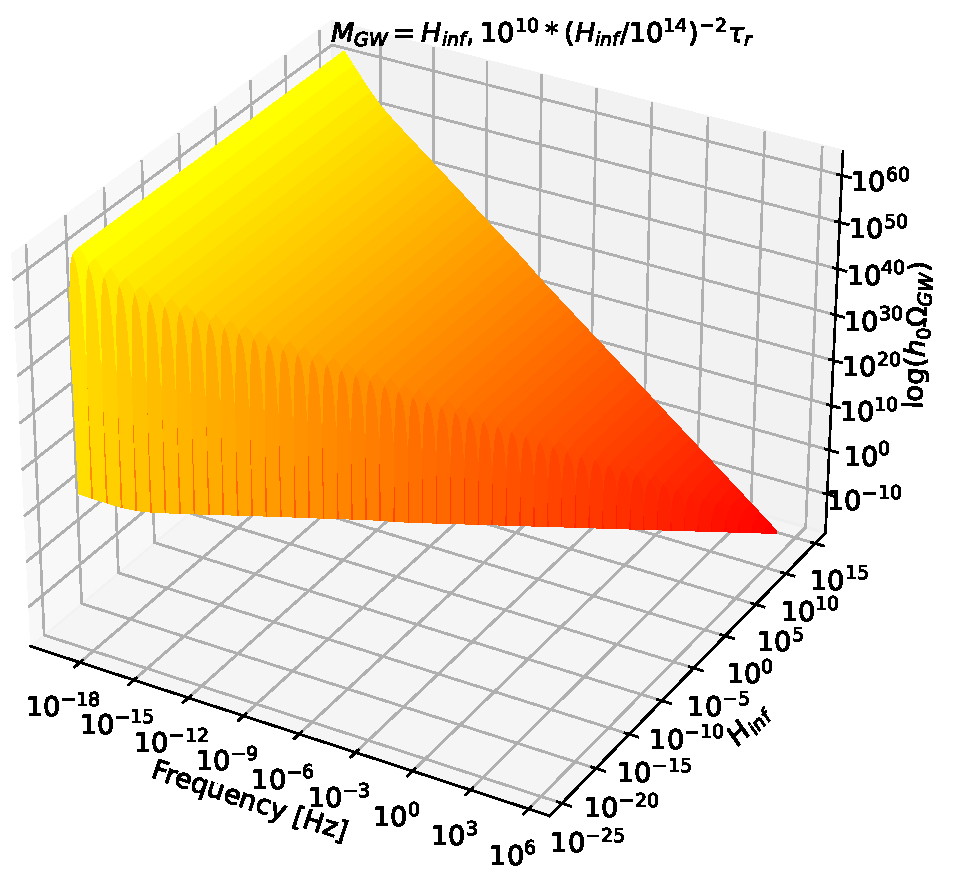
\includegraphics[width=.82\linewidth]{fig/fig4c.pdf}  
  \label{fig:contour-c}
\end{subfigure}
\caption{We plot $\Omega_{GW,0}$ as a function of $f$ and $M, \tau_m, H_{\inf}$ from top to bottom. $f$ ranges from the scale corresponding to matter-radiation inequality ($\sim 3\times10^{-16}$ Hz) to the inflationary UV cutoff ($\sim 2\times 10^8\left(\frac{H_{\inf}}{10^{14} \GeV}\right)^{1/2}$ Hz \cite{Fujita:2018}).} 
\label{fig:contours}
\end{figure}
\hspace{-1em}where $A_T(k_{ref})$ is the amplitude at the reference scale,
\onecolumngrid
\begin{center}
\begin{figure}
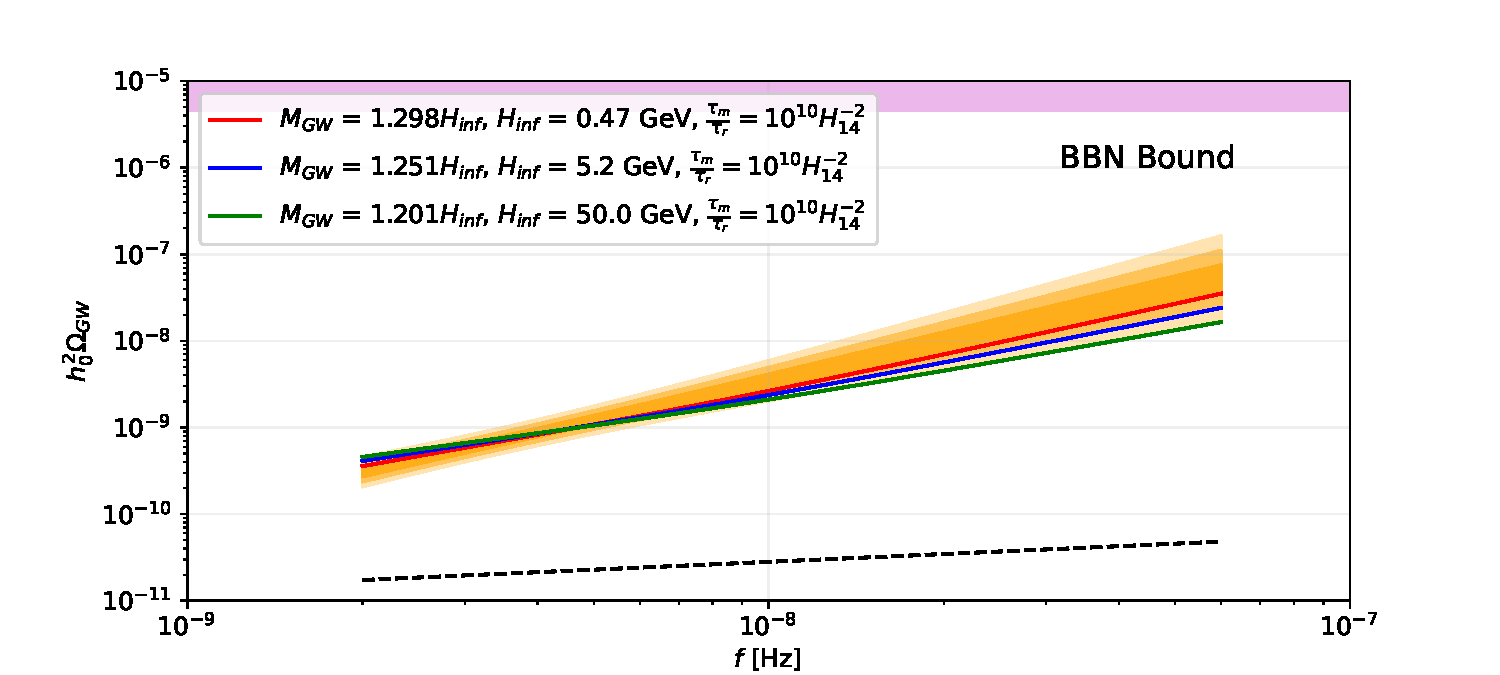
\includegraphics[width=\textwidth]{fig/fig8.pdf} 
\caption{GWB spectra produced by the CM model \cite{Gumrukcuoglu:2012} in the top plot and GWB spectra produced by the SFM model \cite{Fujita:2018} in the bottom plot. We show the $2\sigma$ and $4\sigma$ posterior medians for NG15, in darker and lighter orange respectively. The black dotted lines are the GWB spectrum produced by an astrophysical population of inspiraling SMBHBs with the parameters detailed in Eq.\ A1 of \cite{Afzal:2023}. Top plot (CM): red curve is the energy density for a graviton with the same mass as the upper bound found in \cite{Wang:2023}, the blue curve is the same but for \cite{Wu:2023}, and the green curve is the same but for the NG15 frequency limits. Bottom plot (SFM): blue curve is the GWB spectra fitted to the $2\sigma$ posterior and the red curve is fitted to the $4\sigma$ posterior.}
\label{fig:GWB}
\end{figure}
\end{center}
\twocolumngrid 
\hspace{-1em}measured to be precisely $4.4\times 10^{10}$, and $n_T$ is the spectral index chosen to be 0. The reference scale $k_{ref}$ is chosen to be 0.01 Mpc$\/^{-1}$. $T_{T}$ is defined in Eq.\ 12 of \cite{Kuroyanagi:2015} as follows 
\begin{equation}\label{eqn:24}
    T_T^2(k) = \Omega_m^2 \frac{g_*(T_{in})}{g_{*0}} \frac{g_{*s0}^{4/3}}{g_{*s}^{4/3}(T_{in})} \frac{9j_1^2(k\tau_0)}{(k\tau_0)^2}T_1^2(x_{eq}) T_2^2(x_R)
\end{equation}
where $g_{*}(T_{in})$ and $g_{*0}$ are the relativistic degrees of freedom at the inflation temperature scale and the present respectively, $g_{*s}(T_{in})$ and $g_{*s0}$ are their counterparts for entropy, $j_1(k\tau_0)$ is the 1st spherical Bessel function whose approximation $j_1(k\tau_0) \simeq 1/(\sqrt{2}k\tau_0)$ will be used, the fitting functions are empirically found to be $T_1^2(x) = 1+1.57x+3.42x^2$ and $T_2^2(x) = (1-0.22x^{1.5} + 0.65x^2)^{-1}$, and $x_i \equiv k/k_i$. The values for all of the constants and the forms of the functions are taken from Sec. 2.1 of \cite{Kuroyanagi:2015}. 

Since we are interested in the energy density at the present time, we consider $\Omega_{GW,0}(f) = \Omega_{GW}(\tau_0,f)$, which is now
\begin{equation}\label{eqn:25}
    \Omega_{GW,0}(f) = \frac{\pi^2f^2}{3a_0^2 H_0^2}\frac{\tau_m}{\tau_r}(k\tau_r)^{3-2\nu}\mathcal{P}_{GR}(k) .
\end{equation}
In anticipation of our consideration of certain parameters in the next section, we look at the behavior of the energy density as a function of different parameters. Fig.\ \ref{fig:contours} shows how $\Omega_{GW,0}$ varies with changing $f$ and $M_{GW}, \tau_m$, and $H_{\inf}$. We note that in Fig.\ \ref{fig:contours} for the topmost and bottommost plots where we are not varying $\tau_m$, we are taking the upper bound of $\tau_m$, which is determined by the Big Bang Nucleosynthesis (BBN) bounds and is given by Eq.\ 16 of \cite{Fujita:2018}
\begin{equation}\label{eqn:26}
    \tau_m \lesssim 10^{10}\left(\frac{H_{\inf}}{10^{14} \GeV}\right)^{-2}\tau_r
\end{equation}

\section{Results}
We now discuss the region of the parameter space in the two models that can potentially explain the signals from NG15. 

\subsection{CM}

The constraint on the mass is straightforward in the CM model. We expect a peaked signature in the energy density if the mass is a constant value, as seen in Fig.\ \ref{fig:CM_omega}. We can see that a peaked signature isn't present in the NG15 signal, so no graviton mass in the CM model can possibly explain the NG15 signal. Thus, if the graviton has a non-zero mass, the peak in the energy density of primordial gravitational waves must be below the lower range of the frequency of the NG15 signal. An upper bound based on this consideration is thus equal to $M_{GW} = 8.3\times10^{-33} \GeV/c^2$, since the lowest frequency in the signal is 2 nHz \cite{Agazie:2023}. This is in agreement with the state-of-the-art bounds from Ref.\ \cite{Wu:2023}, which has the upper bound at $M_{GW} = 8.2\times10^{-33} \GeV/c^2$, and from Ref.\ \cite{Wang:2023}, which has the upper bound at $M_{GW} = 8.6\times10^{-33} \GeV/c^2$, as shown in Fig.\ \ref{fig:GWB}.

\subsection{SFM}

The constraints we can place on the SFM model based on NG15 are done by considering the constraints we can place on the parameters $M_{GW}, H_{\inf},$ and $\tau_m$. Based on the contours in Fig.\ \ref{fig:contours}, we were able reproduce the NG15 signal with MG by varying the values for the parameters that lie within $2\sigma$ and $4\sigma$ of the power law posterior of the signal. We assumed that $\tau_m$ took on its maximum value allowed by the BBN bounds, from Eq.\ \ref{eqn:26}, because increasing $\tau_m$ causes the energy density to uniformly increase, which gets us closer to the signal by being as far as we can from violating the Higuchi bound. This came out to be $M_{GW} = 1.14H_{\inf}$ and $H_{\inf} = 500 \GeV$ to stay within $2\sigma$ of the posterior and $M_{GW} = 1.25H_{\inf}$ and $H_{\inf} = 5 \GeV$ to stay within $4\sigma$ of the posterior. 
\begin{figure}[h]
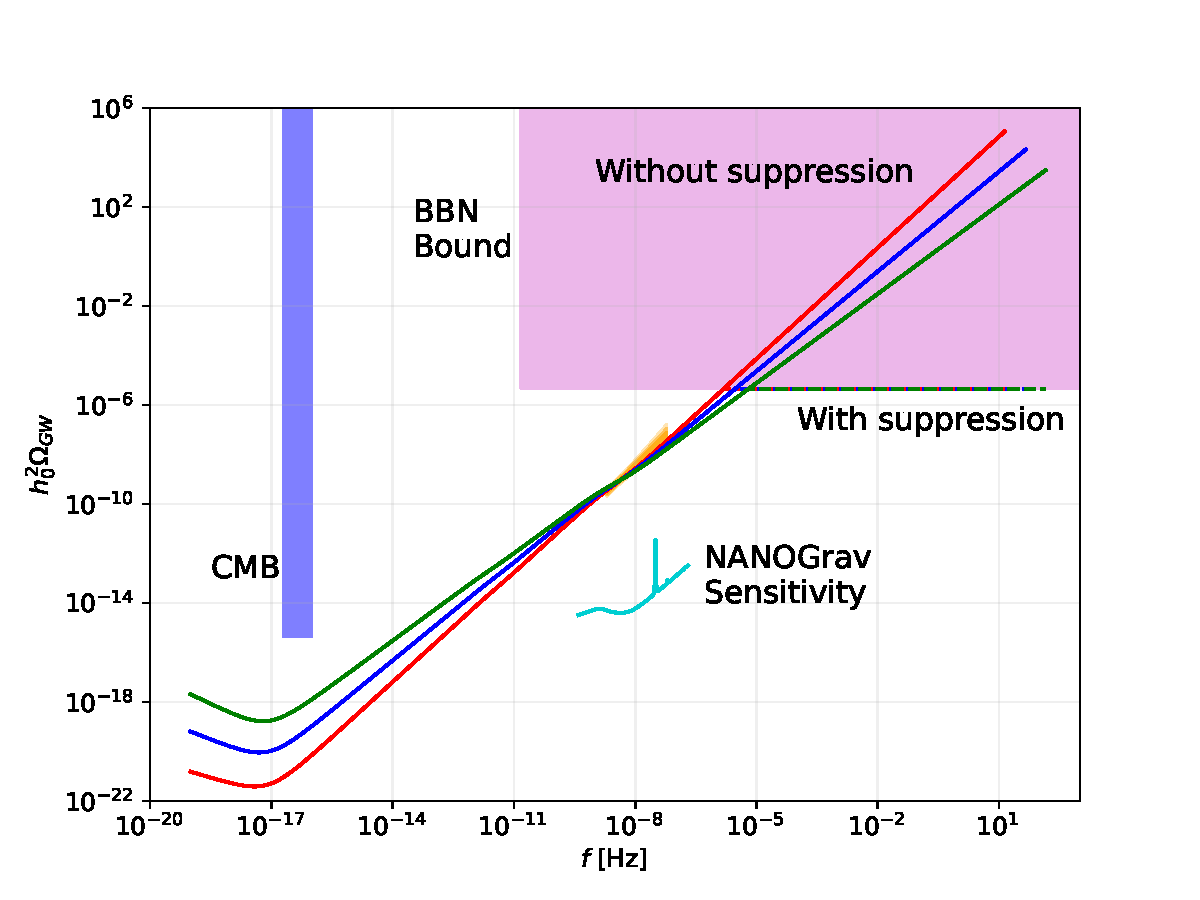
\includegraphics[width=\linewidth]{fig/fig7.pdf}
\caption{The energy densities in the bottom plot of Fig.\ \ref{fig:GWB} plotted over the whole frequency range specified in Fig.\ \ref{fig:contours}.}
\label{fig:bound}
\end{figure}
\section{Discussion}
In this paper, we discussed how the CM and SFM models of MG can be constrained by NG15. We note that the selection of the parameters in the SFM model leads to energy densities that violate the BBN bound for higher frequencies; in the region of frequencies $\gtrsim 10^{-6}$ Hz. We propose that there could be some mechanism that suppresses the energy density of gravitational waves from the primordial era for those frequencies. Something analogous to the damping of the energy density from the free-streaming neutrinos \cite{Weinberg:2004} could be behind such a suppression necessary to respect the BBN bound. 

GW observation has mostly ruled out the possibility of gravitons with a very low but nonzero mass, since the expectation that a peak could be present for lower and lower frequencies is becoming more slim, albeit still possible. Therefore, the more plausible possibility of MG is the scenario in which the graviton mass is a non-constant function of time. We have only considered a step function as the time dependent function, but more complex functions are possible. The mechanism behind such a mass decay would come from the exact nature of the phase transition of the gravitational field itself. It may be interesting to pursue an investigation to place constraints on the specific evolution of the mass during the phase transition. Then, we would be able to probe the mass evolution and shed insight into the time dependent behavior beyond a step function.

\vspace{2mm}
{\bf Data availability}---Source code to reproduce all of the figures in this paper is located in \cite{GH}. 
\vspace{2mm}

{\bf Acknowledgements}---We thank Prof.\ Shinji Mukohyama and Prof.\ Sachiko Kuroyanagi for insightful discussions on the nature of their models.

\bibliographystyle{apsrev4-2_edited}
\bibliography{refs}

%\printbibliography

\clearpage
\end{document}
